
\documentclass{article}

\usepackage[utf8]{inputenc}
\usepackage[T1]{fontenc}
\usepackage{makeidx}
\usepackage{bussproofs}
\usepackage{amsmath,amssymb}
\usepackage{tabularx}
\usepackage{pgf, tikz}
% \usepackage[margin=4cm]{geometry}

\usepackage{float}
\floatstyle{boxed}
\restylefloat{figure}

\usepackage{listings}
\lstset{language=[Objective]caml}

% $Id$

\def\ai{\textsf{Aesthetic~Integration}}
\def\alloy{\textsf{Alloy}}
\def\altergo{\textsf{Alt-Ergo}}
\def\altergoz{\textsf{Alt-Ergo~Zero}}
\def\archsat{\textsf{ArchSAT}}
\def\atelierb{\textsf{Atelier~B}}
\def\bbook{\textsf{B}-Book}
\def\bmth{\textsf{B}}
\def\bware{\textsf{BWare}}
\def\cvc{\textsf{CVC4}}
\def\e{\textsf{E}}
\def\ens{\textsf{ENS Paris-Saclay}}
\def\git{\textsf{Git}}
\def\inria{\textsf{Inria}}
\def\intel{\textsf{Intel~Xeon~E5-1650~v3}}
\def\iproverm{\textsf{iProver~Modulo}}
\def\lirmm{\textsf{LIRMM}}
\def\lsv{\textsf{LSV}}
\def\msat{\textsf{mSAT}}
\def\ocaml{\textsf{OCaml}}
\def\princess{\textsf{Princess}}
\def\um{\textsf{Université de Montpellier}}
\def\vdm{\textsf{VDM}}
\def\satallax{\textsf{Satallax}}
\def\zenm{\textsf{Zenon~Modulo}}
\def\zenon{\textsf{Zenon}}
\def\zipper{\textsf{Zipperposition}}
\def\znot{\textsf{Z}}

\EnableBpAbbreviations{}
\newcommand{\UICm}[1]{\UIC{$#1$}}
\newcommand{\AXCm}[1]{\AXC{$#1$}}
\newcommand{\BICm}[1]{\BIC{$#1$}}
\newcommand{\TICm}[1]{\TIC{$#1$}}
\newcommand{\RLm}[1]{\RL{$#1$}}

\newcommand\clauseWithSubst[2]{\ensuremath{#1 ~|~ #2}}
\newcommand\renameVarsSymb{\ensuremath{\textsf{rename}}}
\newcommand\renameVars[1]{\ensuremath{\renameVarsSymb}(#1)}
\newcommand\mapVar[2]{\ensuremath{ #1 \mapsto #2 }}

\def\rew{\longrightarrow}
\def\arg{\mbox{-}}
\def\type{\textsf{Type}}
\def\omicron{o}
\newcommand\set[1]{\mathsf{set}(#1)}
\newcommand\tuple[2]{\mathsf{tup}(#1,#2)}
\def\plus{\raisebox{.22\height}{\scalebox{.6}{\pmb{+}}}}
\def\fctpart{~{\kern+.2em\mapstochar{}\!\!\!\!\!\rightarrow}~}
\def\injpart{~~{\mapstochar{}\!\!\!\!\!\!\rightarrowtail}~}
\def\surpart{~{\kern+.2em\mapstochar{}\!\!\!\!\!\twoheadrightarrow}~}
\def\bijpart{~{\kern+.1em\mapstochar{}\!\!\!\!\!\rightarrowtail\kern+.03em
\!\!\!\!\!\!\twoheadrightarrow}~}
\def\bijtotal{~{\kern-.1em\rightarrowtail\kern+.03em\!\!\!\!\!\!
\twoheadrightarrow}~}
\def\override{~~{\plus{}\mkern-24mu<}~}
\def\substleft{~{-\mkern-14mu\lhd}~}
\def\substright{~{-\mkern-14mu\rhd}~}

\newlength\memparindent
\setlength{\memparindent}{\parindent}
\newcommand{\myindent}{\hspace{\memparindent}}

\newcommand\todo[1]{\textcolor{red}{#1}}


\usetikzlibrary{arrows, automata}

\begin{document}

\title{\msat{}: a \sat{}/\smt{}/\mcsat{} library}
\author{Guillaume~Bury}

\maketitle

\section{Introduction}

The goal of the \msat{} library is to provide a way to easily
create automated theorem provers based on a \sat{} solver. More precisely,
the library, written in \ocaml{}, provides functors which, once instantiated,
provide a \sat{}, \smt{} or \mcsat{} solver.

Given the current state of the art of \smt{} solvers, where most \sat{} solvers
are written in C and heavily optimised\footnote{Some solvers now have instructions
to manage a processor's cache}, the \msat{} library does not aim to provide solvers
competitive with the existing implementations, but rather an easy way to create
reasonably efficient solvers.

\msat{} currently uses the following techniques:
\begin{itemize}
  \item 2-watch literals scheme
  \item Activity based decisions
  \item Restarts
\end{itemize}

Additionally, \msat{} has the following features:
\begin{itemize}
  \item Local assumptions
  \item Proof/Model output
  \item Adding clauses during proof search
\end{itemize}

\clearpage

\tableofcontents{}

\clearpage

\section{\sat{} Solvers: principles and formalization}\label{sec:sat}

\subsection{Idea}

\subsection{Inference rules}\label{sec:trail}

The SAT algorithm can be formalized as follows. During the search, the solver keeps
a set of clauses, containing the problem hypotheses and the learnt clauses, and
a trail, which is the current ordered list of assumptions and/or decisions made by
the solver.

Each element in the trail (decision or propagation) has a level, which is the number of decision
appearing in the trail up to (and including) it. So for instance, propagations made before any
decisions have level $0$, and the first decision has level $1$. Propagations are written
$a \leadsto_C \top$, with $C$ the clause that caused the propagation, and decisions
$a \mapsto_n \top$, with $n$ the level of the decision. Trails are read
chronologically from left to right.

In the following, given a trail $t$ and an atomic formula $a$, we will use the following notation:
$a \in t$ if $a \mapsto_n \top$ or $a \leadsto_C \top$ is in $t$, i.e.~$a \in t$ is $a$ is true
in the trail $t$. In this context, the negation $\neg$ is supposed to be involutive
(i.e.~$\neg \neg a = a$), so that, if $a \in t$ then $\neg \neg a = a \in t$.

There exists two main \sat{} algorithms: \dpll{} and \cdcl{}. In both, there exists
two states: first, the starting state $\text{Solve}$, where propagations
and decisions are made, until a conflict is detected, at which point the algorithm
enters in the $\text{Analyse}$ state, where it analyzes the conflict, backtracks,
and re-enter the $\text{Solve}$ state. The difference between \dpll{} and \cdcl{}
is the treatment of conflicts during the $\text{Analyze}$ phase: \dpll{} will use
the conflict only to known where to backtrack/backjump, while in \cdcl{} the result
of the conflict analysis will be added to the set of hypotheses, so that the same
conflict does not occur again.
The $\text{Solve}$ state take as argument the set of hypotheses and the trail, while
the $\text{Analyze}$ state also take as argument the current conflict clause.

We can now formalize the \cdcl{} algorithm using the inference rules
in Figure~\ref{fig:smt_rules}. In order to completely recover the \sat{} algorithm,
one must apply the rules with the following precedence and termination conditions,
depending on the current state:
\begin{itemize}
  \item If the empty clause is in $\mathbb{S}$, then the problem is unsat.
    If there is no more rule to apply, the problem is sat.
  \item If we are in $\text{Solve}$ mode:
    \begin{enumerate}
      \item First is the rule \irule{Conflict};
      \item Then the try and use \irule{Propagate};
      \item Finally, is there is nothing left to be propagated, the \irule{Decide}
        rule is used.
    \end{enumerate}
  \item If we are in $\text{Analyze}$ mode, we have a choice concerning
    the order of application. First we can observe that the rules
    \irule{Analyze-Propagate}, \irule{Analyze-Decision} and \irule{Analyze-Resolution}
    can not apply simultaneously, and we will thus group them in a super-rule
    \irule{Analyze}. We now have the choice of when to apply the \irule{Backjump} rule
    compared to the \irule{Analyze} rule:
    using \irule{Backjump} eagerly will result in the first UIP strategy, while delaying it
    until later will yield other strategies, both of which are valid.
\end{itemize}

\begin{figure}
  \center{\underline{\sat{}}}
  \begin{center}
    \begin{tabular}{c@{\hspace{1cm}}l}
      % Propagation (boolean)
      \AXC{$\text{Solve}(\mathbb{S}, t)$}
      \LLc{Propagate}
      \UIC{$\text{Sove}(\mathbb{S}, t :: a \leadsto_C \top)$}
      \DP{} &
      \begin{tabular}{l}
        $a \in C, C \in \mathbb{S}, \neg a \notin t$ \\
        $\forall b \in C. b \neq a \rightarrow \neg b \in t$ \\
      \end{tabular}
      \\ \\
      % Decide (boolean)
      \AXC{$\text{Solve}(\mathbb{S}, t)$}
      \LLc{Decide}
      \UIC{$\text{Solve}(\mathbb{S}, t :: a \mapsto_n \top)$}
      \DP{} &
      \begin{tabular}{l}
        $a \notin t, \neg a \notin t, a \in \mathbb{S}$ \\
        $n = \text{max\_level}(t) + 1$ \\
      \end{tabular}
      \\ \\
      % Conflict (boolean)
      \AXC{$\text{Solve}(\mathbb{S}, t)$}
      \LLc{Conflict}
      \UIC{$\text{Analyze}(\mathbb{S}, t, C)$}
      \DP{} &
      $C \in \mathbb{S}, \forall a \in C. \neg a \in t$
      \\ \\
    \end{tabular}
  \end{center}
  \begin{center}
    \begin{tabular}{c@{\hspace{.5cm}}l}
      % Analyze (propagation)
      \AXC{$\text{Analyze}(\mathbb{S}, t :: a \leadsto_C \top, D)$}
      \LLc{Analyze-propagation}
      \UIC{$\text{Analyze}(\mathbb{S}, t, D)$}
      \DP{} &
      $\neg a \notin D$
      \\ \\
      % Analyze (decision)
      \AXC{$\text{Analyze}(\mathbb{S}, t :: a \mapsto_n \top, D)$}
      \LLc{Analyze-decision}
      \UIC{$\text{Analyze}(\mathbb{S}, t, D)$}
      \DP{} &
      $\neg a \notin D$
      \\ \\
      % Resolution
      \AXC{$\text{Analyze}(\mathbb{S}, t :: a \leadsto_C \top, D)$}
      \LLc{Analyze-Resolution}
      \UIC{$\text{Analyze}(\mathbb{S}, t, (C - \{a\}) \cup (D - \{ \neg a\}))$}
      \DP{} &
      $\neg a \in D$
      \\ \\
    \end{tabular}
  \end{center}
  \begin{center}
    \begin{tabular}{c@{\hspace{1cm}}l}
      % BackJump
      \AXC{$\text{Analyze}(\mathbb{S}, t :: a \mapsto_d \top :: t', C)$}
      \LLc{Backjump}
      \UIC{$\text{Solve}(\mathbb{S} \cup \{ C \}, t)$}
      \DP{} &
      \begin{tabular}{l}
        $\text{is\_uip}(C, t :: a \mapsto_d \top :: t')$ \\
        $d \leq \text{uip\_level}(C)$ \\
      \end{tabular}
      \\ \\
    \end{tabular}
  \end{center}

  \center{\underline{\smt{}}}
  \begin{center}
    \begin{tabular}{c@{\hspace{1cm}}l}
      % Conflict (theory)
      \AXC{$\text{Solve}(\mathbb{S}, t)$}
      \LLc{Smt}
      \UIC{$\text{Solve}(\mathbb{S} \cup \{C\}, t)$}
      \DP{} &
      \begin{tabular}{l}
        $\mathcal{T} \vdash C$ \\
      \end{tabular}
      \\ \\
    \end{tabular}
  \end{center}
  \caption{Inference rules for \sat{} and \smt{}}\label{fig:smt_rules}
\end{figure}


\subsection{Invariants, correctness and completeness}

The following invariants are maintained by the inference rules in Figure~\ref{fig:smt_rules}:
\begin{description}
  \item[Trail Soundness] In $\text{Solve}(\mathbb{S}, t)$, if $a \in t$ then $\neg a \notin t$
  \item[Conflict Analysis] In $\text{Analyze}(\mathbb{S}, t, C)$, $C$ is a clause implied by the
    clauses in $\mathbb{S}$, and $\forall a \in C. \neg a \in t$ (i.e.~$C$ is entailed by the
    hypotheses, yet false in the partial model formed by the trail $t$).
  \item[Equivalence] In any rule \AXC{$s_1$}\UIC{$s_2$}\DP{}, the set of hypotheses
    (usually written $\mathbb{S}$) in $s_1$ is equivalent to that of $s_2$.
\end{description}

These invariants are relatively easy to prove, and provide an easy proof of correctness for
the \cdcl{} algorithm. Termination can be proved by observing that the same trail appears
at most twice during proof search (once during propagation, and eventually a second time
right after backjumping\footnote{This could be avoided by making the \irule{Backjump} rule
directly propagate the relevant literal of the conflict clause, but it needlessly
complicates the rule.}). Correctness and termination implies completeness of the \sat{}
algorithm.


\section{\smt{} solver architecture}\label{sec:smt}

\subsection{Idea}\label{sec:smt_flow}

In a \smt{} solver, after each propagation and decision, the solver sends the newly
assigned literals to the theory. The theory then has the possibility to declare the
current set of literals incoherent, and give the solver a tautology in which all
literals are currently assigned to $\bot$\footnote{or rather for each literal, its negation
is assigned to $\top$}, thus prompting the solver to backtrack.
We can represent a simplified version of the information flow (not taking into
account backtracking) of usual \smt{} Solvers, using the graph in fig~\ref{fig:smt_flow}.

Contrary to what the Figure~\ref{fig:smt_flow} could suggest, it is not impossible
for the theory to propagate information back to the \sat{} solver. Indeed,
some \smt{} solvers already allow the theory to propagate entailed literals back to the
\sat{} solver. However, these propagations are in practice limited by the complexity
of deciding entailment. Moreover, procedures in a \smt{} solver should be incremental
in order to get decent performances, and deciding entailment in an incremental manner
is not easy (TODO~: ref nécessaire). Doing efficient, incremental entailment is exactly
what \mcsat{} allows (see Section~\ref{sec:mcsat}).

\subsection{Formalization and Theory requirements}

An \smt{} solver is the combination of a \sat{} solver, and a theory $\mathcal{T}$.
The role of the theory $\mathcal{T}$ is to stop the proof search as soon as the trail
of the \sat{} solver is inconsistent. A trail is inconsistent iff there exists a clause
$C$, which is a tautology of $\mathcal{T}$ (thus $\mathcal{T} \vdash C$), but is not
satisfied in the current trail (each of its literals has either been decided or
propagated to false).

TODO:reword the following paragraph (inference rule Conflict-SMT renamed to SMT)

Thus, we can add the \irule{Conflict-Smt} rule (see
Figure~\ref{fig:smt_rules}) to the \cdcl{} inference rules in order to get a \smt{} solver.
We give the \irule{Conflict-Smt} rule a slightly lower precedence than the
\irule{Conflict} rule for performance reason (detecting boolean conflict is
faster than theory specific conflicts).

So, what is the minimum that a theory must implement in practice to be used in a
\smt{} solver~? The theory has to ensure that the current trail is consistent
(when seen as a conjunction of literals), that is to say, given a trail $t$,
it must ensure that there exists a model $\mathcal{M}$ of $\mathcal{T} $so that
$\forall a \in t. \mathcal{M} \vDash a$, or if it is impossible (i.e.~the trail
is inconsistent) produce a conflict.

\begin{figure}
  \begin{center}
    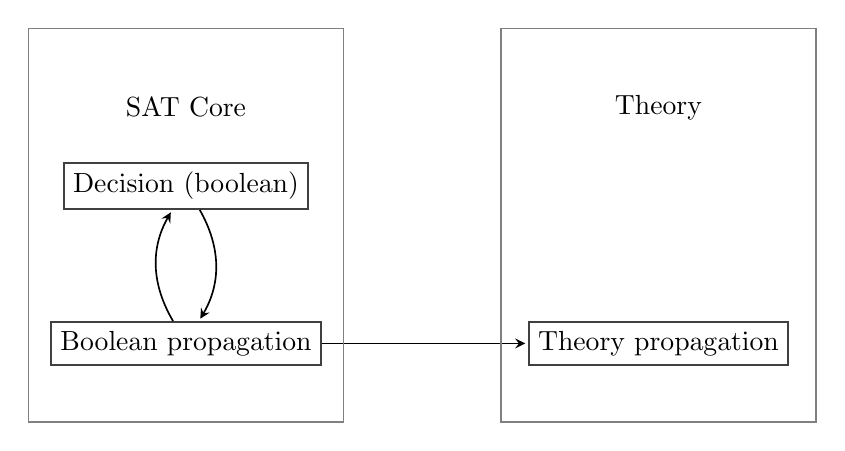
\begin{tikzpicture}[
        ->, % Arrow style
        > = stealth, % arrow head style
        shorten > = 1pt, % don't touch arrow head to node
        node distance = 2cm, % distance between nodes
        semithick, % line style
        auto
      ]

      \tikzstyle{state}=[rectangle,draw=black!75]

      \node (sat) {SAT Core};
      \node (th) [right of=sat, node distance=6cm] {Theory};
      \node[state] (d) [below of=sat, node distance=1cm] {Decision (boolean)};
      \node[state] (bp) [below of=d, node distance=2cm] {Boolean propagation};
      \node[state] (tp) [right of=bp, node distance=6cm] {Theory propagation};

      \draw (d) edge [bend left=30] (bp);
      \draw (bp) edge [bend left=30] (d);
      \draw (bp) edge (tp);

      \draw[black!50] (-2,1) rectangle (2,-4);
      \draw[black!50] (4,1) rectangle (8,-4);

    \end{tikzpicture}
  \end{center}
  \caption{Simplified \smt{} Solver architecture}\label{fig:smt_flow}
\end{figure}

\section{\mcsat{}: An extension of \smt{} Solvers}\label{sec:mcsat}

\subsection{Motivation and idea}

\mcsat{} is an extension of usual \smt{} solvers, introduced in~\cite{VMCAI13} and~\cite{FMCAD13}.
In usual \smt{} Solvers, interaction between the core SAT Solver and the Theory is pretty limited~:
the SAT Solver make boolean decisions and propagations, and sends them to the theory,
whose role is in return to stop the SAT Solver as soon as the current set of assumptions
is incoherent. This means that the information that theories can give the SAT Solver is
pretty limited, and furthermore it heavily restricts the ability of theories to guide
the proof search (see Section~\ref{sec:smt_flow}).

While it appears to leave a reasonably simple job to the theory, since it completely
hides the propositional structure of the problem, this simple interaction between the
SAT Solver and the theory makes it harder to combine multiple theories into one. Usual
techniques for combining theories in \smt{} solvers typically require to keep track of
equivalence classes (with respect to the congruence closure) and for instance
in the Nelson-Oppen method for combining theories (TODO~: ref nécessaire) require of
theories to propagate any equality implied by the current assertions.

\mcsat{} extends the SAT paradigm by allowing more exchange of information between the theory
and the SAT Solver. This is achieved by allowing the solver to not only decide on the truth value
of atomic propositions, but also to decide assignments for terms that appear in the problem.
For instance, if the SAT Solver assigns a variable $x$ to $0$,
an arithmetic theory could propagate to the SAT Solver that the formula $x < 1$ must also hold,
instead of waiting for the SAT Solver to guess the truth value of $x < 1$ and then
inform the SAT Solver that the conjunction~: $x = 0 \land \neg x < 1$ is incoherent.

This exchange of information between the SAT Solver and the theories results in
the construction of a model throughout the proof search (which explains the name
Model Constructing SAT).

The main addition of \mcsat{} is that when the solver makes a decision, instead of
being restricted to making boolean assignment of formulas, the solver now can
decide to assign a value to a term belonging to one of the literals. In order to do so,
the solver first chooses a term that has not yet been assigned, and then asks
the theory for a possible assignment. Like in usual SMT Solvers, a \mcsat{} solver
only exchange information with one theory, but, as we will see, combination
of theories into one becomes easier in this framework, because assignments are
actually a very good way to exchange information.

Using the assignments on terms, the theory can then very easily do efficient
propagation of formulas implied by the current assignments: it is enough to
evaluate formulas using the current partial assignment.
The information flow then looks like fig~\ref{fig:mcsat_flow}.

\begin{figure}
  \begin{center}
    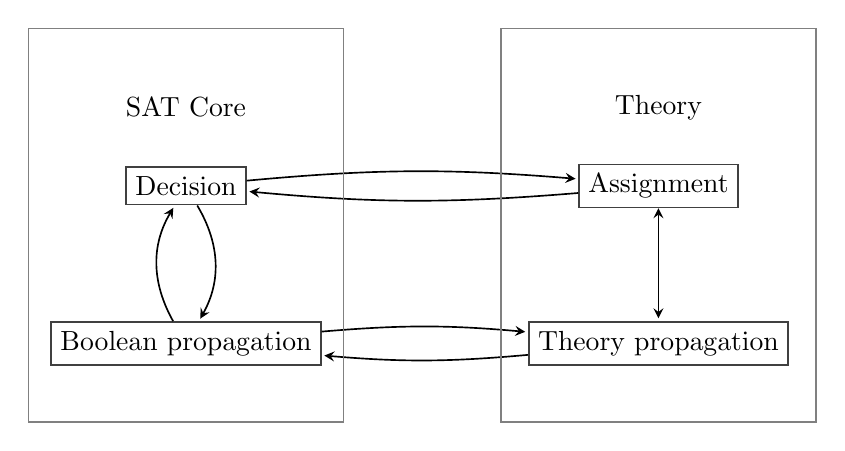
\begin{tikzpicture}[
        ->, % Arrow style
        > = stealth, % arrow head style
        shorten > = 1pt, % don't touch arrow head to node
        node distance = 2cm, % distance between nodes
        semithick, % line style
        auto
      ]

      \tikzstyle{state}=[rectangle,draw=black!75]

      \node (sat) {SAT Core};
      \node (th) [right of=sat, node distance=6cm] {Theory};
      \node[state] (d) [below of=sat, node distance=1cm] {Decision};
      \node[state] (ass) [right of=d, node distance=6cm] {Assignment};
      \node[state] (bp) [below of=d, node distance=2cm] {Boolean propagation};
      \node[state] (tp) [right of=bp, node distance=6cm] {Theory propagation};

      \draw (bp)[right] edge [bend left=5] (tp);
      \draw (tp) edge [bend left=5] (bp);
      \draw (bp) edge [bend left=30] (d);
      \draw (ass) edge [bend left=5] (d);
      \draw (d) edge [bend left=5] (ass);
      \draw (d) edge [bend left=30] (bp);
      \draw[<->] (ass) edge (tp);

      \draw[black!50] (-2,1) rectangle (2,-4);
      \draw[black!50] (4,1) rectangle (8,-4);

    \end{tikzpicture}
  \end{center}
  \caption{Simplified \mcsat{} Solver architecture}\label{fig:mcsat_flow}
\end{figure}

\subsection{Decisions and propagations}

In \mcsat{}, semantic propagations are a bit different from the propagations
used in traditional \smt{} Solvers. In the case of \mcsat{} (or at least the version presented here),
semantic propagations strictly correspond to the evaluation of formulas in the
current assignment. Moreover, in order to be able to correctly handle these semantic
propagations during backtrack, they are assigned a level: each decision is given a level
(using the same process as in a \sat{} solvers: a decision level is the number of decision
previous to it, plus one), and a formula is propagated at the maximum level of the decisions
used to evaluate it.

We can thus extend the notations introduced in Section~\ref{sec:trail}: $t \mapsto_n v$ is
a semantic decision which assign $t$ to a concrete value $v$, $a \leadsto_n \top$ is a
semantic propagation at level $n$.

For instance, if the current trail is $\{x \mapsto_1 0, x + y + z = 0 \mapsto_2 \top, y\mapsto_3 0\}$,
then $x + y = 0$ can be propagated at level $3$, but $z = 0$ can not be propagated, because
$z$ is not assigned yet, even if there is only one remaining valid value for $z$.
The problem with assignments as propagations is that it is not clear what to do with
them during the $\text{Analyze}$ phase of the solver, see later.

\begin{figure}
  \begin{center}
    \begin{align*}
      \text{max\_level}([]) &= 0 \\
      \text{max\_level}(t :: a \mapsto_n \top) &= n \\
      \text{max\_level}(t :: a \leadsto_C \top) &= \text{max\_level}(t) \\
      \text{level}(a, t :: a \mapsto_n \top :: t')  &= n \\
      \text{level}(a, t :: a \leadsto_C \top :: t') &= \text{max\_level}(t) \\
    \end{align*}
    \begin{align*}
      \text{max\_lit}(a, C, t) &= \forall b \in C, (b \neq a) \rightarrow
                                    \text{level}(b, t) < n \\
      \text{is\_uip}(C, t) &= \exists (a \mapsto_n \top) \in t,
                                a \in C \land \text{max\_lit}(a, C, t) \\
      \text{uip\_level}(C, t) = l &\equiv \exists (a \mapsto_n \top) \in t,
                                            a \in C \land \text{max\_lit}(a, C, t)
                                            \land l = \text{max\_level}(C, t) \\
    \end{align*}
  \end{center}
  \caption{}\label{fig:analyze_functions}
\end{figure}


\subsection{First order terms \& Models}

A model traditionally is a triplet which comprises a domain,
a signature and an interpretation function. Since most problems, do not
define new interpreted functions or constants\footnote{Indeed, thses typically
only come from built-in theories such as arithmetic, bit-vectors, etc\ldots},
and built-in theories such as arithmetic usually have canonic domain and signature,
we will consider in the following that the domain $\mathbb{D}$, signature, and
intepretation of theory-defined symbols are given and constant. For instance,
there exists more than one first order model of Peano arithmetic (ref nécessaire);
in our case we want to choose one of them, and try and extand it to satisfy the
input problem, but we do not want to try and switch model during the proof search.

In the following, we use the following notations:
\begin{itemize}
  \item $\mathbb{V}$ is an infinite set of variables;
  \item $\mathbb{C}$ is the possibly infinite set of constants defined
    by the input problem's theories\footnote{For instance, the theory of arithmetic
    defines the usual operators $+, -, *, /$ as well as $0, -5, \frac{1}{2}, -2.3, \ldots$};
  \item $\mathbb{S}$ is the finite set of constants defined by the input problem's type
    definitions;
  \item $\mathbb{T}$ is the (infinite) set of first-order terms over $\mathbb{V}$, $\mathbb{C}$
    and $\mathbb{S}$ (for instance $a, f(0), x + y, \ldots$);
  \item $\mathbb{F}$ is the (infinite) set of first order quantified formulas
    over the terms in $\mathbb{T}$.
\end{itemize}

An interpretation $\mathcal{I}$ is a mapping from $\mathbb{V} \cup \mathbb{C} \cup \mathbb{S}$
to $\mathbb{D}$. What we are interested in, is finding an interpretation of a problem, and more
specifically an interpretation of the symbols in $\mathbb{S}$ not defined by
the theory, i.e.~non-interpreted functions.
An interpretation $\mathcal{I}$ can easily be extended to a function from ground terms
and formulas to model value by recursively applying it:
\[
  \mathcal{I}( f ( e_1, \ldots, e_n ) ) =
  \mathcal{I}_f ( \mathcal{I}(e_1), \ldots, \mathcal{I}(e_n) ) \\
\]

TODO:~What do we do with quantified variables~?
What kind of model do we want for these~?

\paragraph{Partial Interpretation}
The goal of \mcsat{} is to construct a first-order model of the input formulas. To do so,
it has to build what we will call partial interpretations: intuitively, a partial
interpretation is a partial function from the constants symbols to the model values.
It is, however, not so simple: during proof search, the \mcsat{} algorithm maintains
a partial mapping from expressions to model values (and not from constant symbols
to model values). The intention of this mapping is to represent a set of constraints
on the partial interpretation that the algorithm is building.
For instance, given a function symbol $f$ of type $(\text{int} \rightarrow \text{int})$ and an
integer constant $a$, one such constraint that we would like to be able to express in
our mapping is the following: $f(a) \mapsto 0$, regardless of the values that $f$ takes on
other argument, and also regardless of the value mapped to $a$. To that end we introduce
the notion of abstract partial interpretation.

An abstract partial interpretation $\sigma$ is a mapping from ground expressions to model values.
To each abstract partial interpretation correspond a set of complete models that realize it.
More precisely, any mapping $\sigma$ can be completed in various ways, leading to a set of
potential interpretations:
\[
  \text{Complete}(\sigma) =
    \left\{
      \mathcal{I}
      \; | \;
      \forall t \mapsto v \in \sigma , \mathcal{I} ( t ) = v
    \right\}
\]

\paragraph{Coherence}
An abstract partial interpretation $\sigma$ is said to be coherent iff
there exists at least one model that completes it,
i.e.~$\text{Complete}(\sigma) \neq \emptyset$. One example
of incoherent abstract partial interpretation is the following
mapping:
\[
  \sigma = \left\{
    \begin{matrix}
      a \mapsto 0 \\
      b \mapsto 0 \\
      f(a) \mapsto 0 \\
      f(b) \mapsto 1 \\
    \end{matrix}
  \right.
\]

\paragraph{Compatibility}
In order to do semantic propagations, we want to have some kind of notion
of evaluation for abstract partial interpretations, and we thus define the
partial interpretation function in the following way:
\[
  \forall t \in \mathbb{T} \cup \mathbb{F}. \forall v \in \mathbb{D}.
  \left(
    \forall \mathcal{I} \in \text{Complete}(\sigma).
    \mathcal{I}(t) = v
  \right) \rightarrow
    \sigma(t) = v
\]

The partial interpretation function is the intersection of the interpretation
functions of all the completions of $\sigma$, i.e.~it is the interpretation
where all completions agree. We can now say that a mapping $\sigma$ is compatible
with a trail $t$ iff $\sigma$ is coherent, and
$\forall a \in t. \neg (\sigma(a) = \bot)$, or in other words, for every literal $a$
true in the trail, there exists at least one model that completes $\sigma$ and where
$a$ is satisfied.

\paragraph{Completeness}
We need one last property on abstract partial interpretations, which is to
specify the relation between the terms in a mapping, and the terms it can evaluate,
according to its partial interpretation function defined above. Indeed, at the end
of proof search, we want all terms (and sub-terms) of the initial problem to be
evaluated using the final mapping returned by the algorithm when it finds that the
problem is satisfiable: that is what we will call completeness of a mapping.
To that end we will here enumerate some sufficient conditions on the mapping domain
$\text{Dom}(\sigma)$ compared to the finite set of terms (and sub-terms) $T$ that
appear in the problem.

A first way, is to have $\text{Dom}(\sigma) = T$, i.e.~all terms (and sub-terms) of the
initial problem are present in the mapping. While this is the simplest way to ensure that
the mapping is complete, it might be a bit heavy: for instance, we might have to assign
both $x$ and $2x$, which is redundant. The problem in that case is that we try and assign
a term for which we could actually compute the value from its arguments: indeed,
since the multiplication is interpreted, we do not need to interpret it in our mapping.
This leads to another way to have a complete mapping: if $\text{Dom}(\sigma)$ is the
set of terms of $T$ whose head symbol is uninterpreted (i.e.~not defined by the theory),
it is enough to ensure that the mapping is complete, because the theory will automatically
constrain the value of terms whose head symbol is interpreted.

\subsection{Inference rules}

\begin{figure}
  \center{\underline{\mcsat{}}}
  \begin{center}
    \begin{tabular}{c@{\hspace{.2cm}}l}
      % Decide (assignment)
      \AXC{$\text{Solve}(\mathbb{S}, t)$}
      \LLc{Theory-Decide}
      \UIC{$\text{Solve}(\mathbb{S}, t :: a \mapsto_n v)$}
      \DP{} &
      \begin{tabular}{l}
        $a \mapsto_k \_ \notin t$ \\
        $n = \text{max\_level}(t) + 1$ \\
        $\sigma_{t :: a \mapsto_n v} \text{ compatible with } t$
      \end{tabular}
      \\ \\
      % Propagation (semantic)
      \AXC{$\text{Solve}(\mathbb{S}, t)$}
      \LLc{Propagate-Theory}
      \UIC{$\text{Solve}(\mathbb{S}, t :: a \leadsto_n \top)$}
      \DP{} &
      $\sigma_t(a) = \top$
      \\ \\
      % Conflict (semantic)
      \AXC{$\text{Solve}(\mathbb{S}, t)$}
      \LLc{Conflict-Mcsat}
      \UIC{$\text{Analyze}(\mathbb{S}, t, C)$}
      \DP{} &
      \begin{tabular}{l}
        $\mathcal{T} \vdash C$ \\
        $\forall a \in C, \neg a \in t \lor \sigma_t(a) = \bot$
      \end{tabular}
      \\ \\
    \end{tabular}
  \end{center}
  \begin{center}
    \begin{tabular}{c@{\hspace{.2cm}}l}
      % Analyze (assign)
      \AXC{$\text{Analyze}(\mathbb{S}, t :: a \mapsto_n v, C)$}
      \LLc{Analyze-Assign}
      \UIC{$\text{Analyze}(\mathbb{S}, t, C)$}
      \DP{} &
      \\ \\
      % Analyze (semantic)
      \AXC{$\text{Analyze}(\mathbb{S}, t :: a \leadsto_n \top, C)$}
      \LLc{Analyze-Semantic}
      \UIC{$\text{Analyze}(\mathbb{S}, t, C)$}
      \DP{} &
      \\ \\
    \end{tabular}
  \end{center}
  \begin{center}
    \begin{tabular}{c@{\hspace{.2cm}}l}
      % Backjump (semantic)
      \AXC{$\text{Analyze}(\mathbb{S}, t :: a \mapsto_n \_ :: \_, C)$}
      \LLc{Backjump-Semantic}
      \UIC{$\text{Solve}(\mathbb{S}, t)$}
      \DP{} &
      \begin{tabular}{l}
        $\text{is\_semantic}(C)$ \\
        $n = \text{slevel}(C)$ \\
      \end{tabular}
      \\ \\
    \end{tabular}
  \end{center}
  \caption{\mcsat{} specific inference rules}\label{fig:mcsat_rules}
\end{figure}

In \mcsat{}, a trail $t$ contains boolean decision and propagations as well as semantic
decisions (assignments) and propagations. We can thus define $\sigma_t$ as the mapping
formed by all assignments in $t$. This lets us define the last rules in Figure~\ref{fig:mcsat_rules},
that, together with the other rules, define the \mcsat{} algorithm.


\bibliographystyle{plain}
\bibliography{biblio}

\clearpage
\appendix

\end{document}
